%ID: 61247
% \begin{blocksection}
\question 61b and 70 are playing a friendly game of RateMyClass and decide to use a  minimax game tree to determine the next optimal move to make. Here 61b wants to get the best possible final rating (maximizer nodes), while 70 is trying to bring it down (minimizer nodes).

\begin{center}
    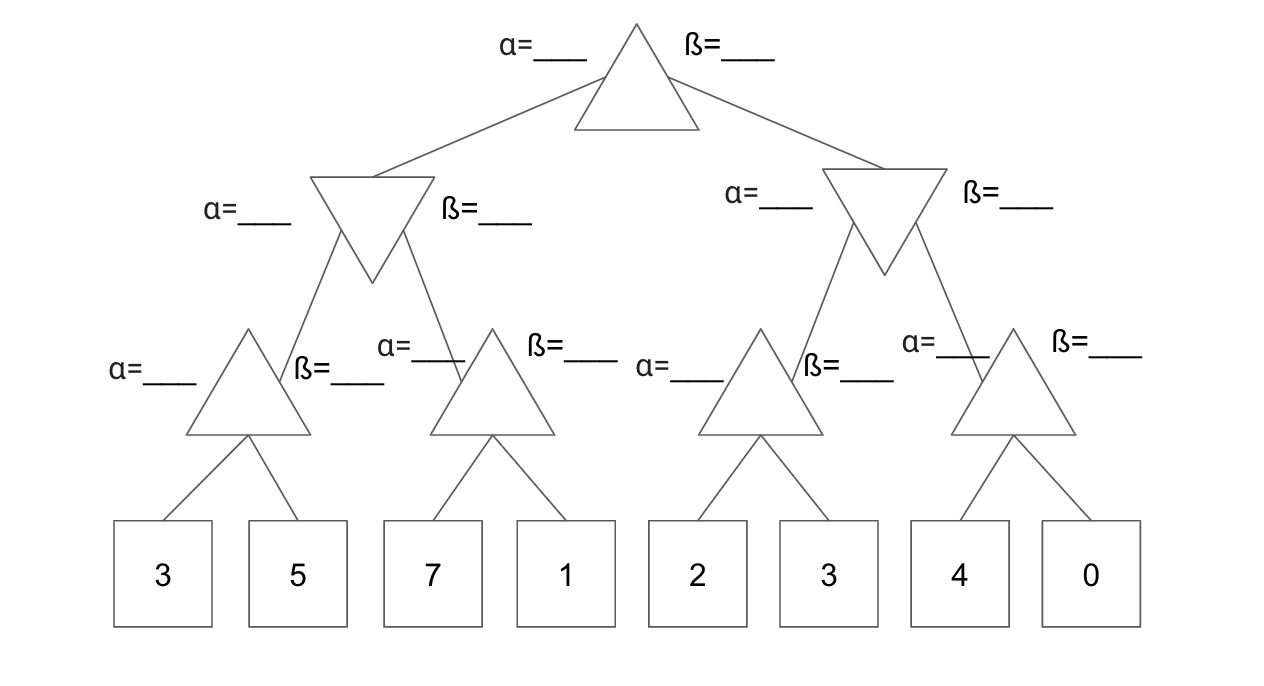
\includegraphics[width=.9\textwidth,height=.9\textheight,keepaspectratio]{topics/trees/game-trees/empty-minimax.png} \newline
\end{center}

\begin{parts}
\item Fill in the values of the game tree to determine the best rating 61b can achieve in this game.

\ifprintanswers
\begin{solution}[2in]
\begin{center}
    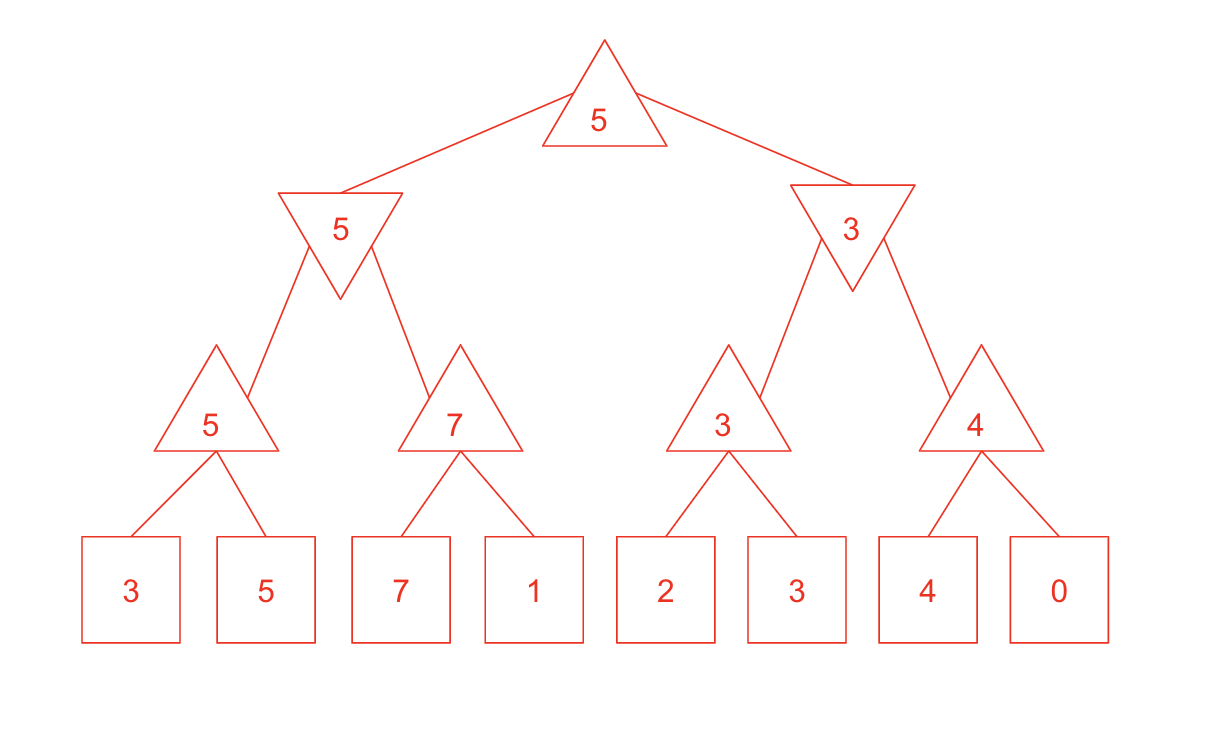
\includegraphics[width=.9\textwidth,height=.9\textheight,keepaspectratio]{topics/trees/game-trees/filled-minimax.png} \newline
 
\end{center}
\end{solution}
\fi


\item 61b knows there is an optimization to the minimax algorithm, and takes advantage of alpha-beta pruning. Which nodes can 61b prune using this algorithm? If no nodes can be pruned explain why not. Assume alpha-beta pruning runs left to right.

\ifprintanswers
\begin{solution}[2in]
\begin{center}
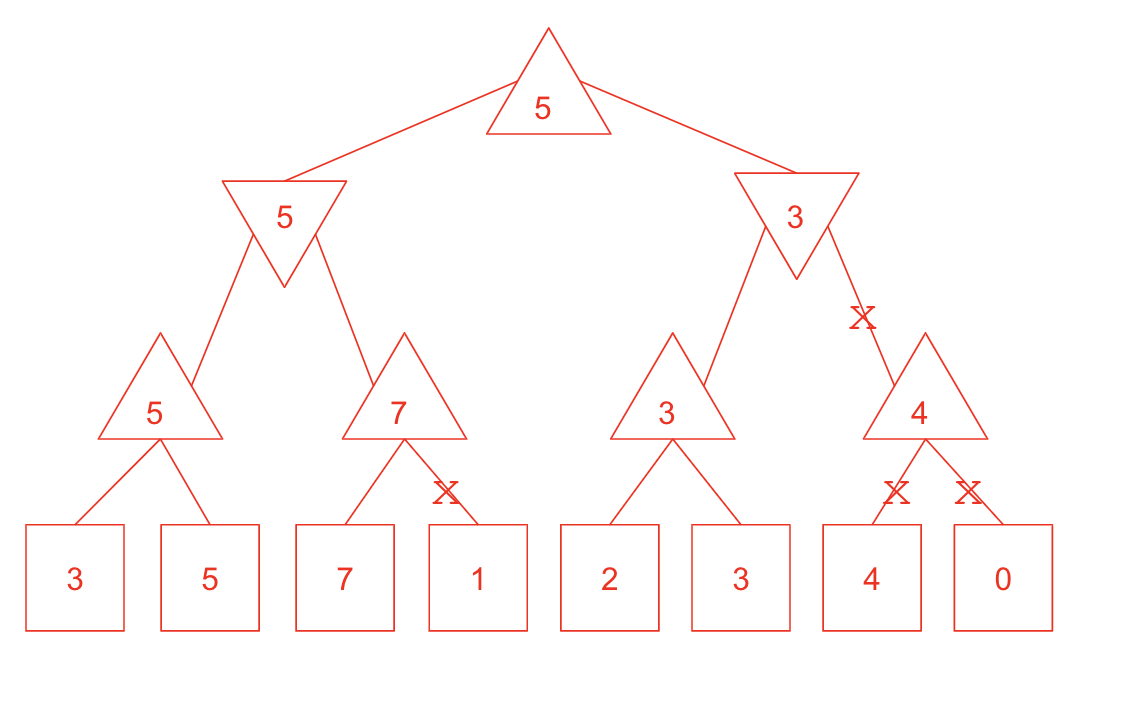
\includegraphics[width=0.85\textwidth]{topics/trees/game-trees/pruned-minimax.png} \newline
\end{center}
\end{solution}
\fi

\item 70 tries to thwart 61b's efforts at pruning and changes the values of Nodes 5-8 (the 4 rightmost leaf nodes) to minimize the number of nodes that can be pruned. Give an example of the modified tree 70 creates. Does this help 70 lower 61b's final rating? (Assume ties are broken by selecting the left node)

\ifprintanswers
\begin{solution}[2in]
Nodes 5 and 6- at least one of them is greater than or equal to 6.

Nodes 7 and 8- at least one of them is greater than or equal to 5

No, this actually helps 61b- its final score will either remain the same, or increase.
\end{solution}
\fi

\end{parts}


% \end{blocksection}